\begin{wrapfigure}[10]{r}[0pt]{105mm}
    \begin{subfigure}[h!]{0.3\textwidth}
        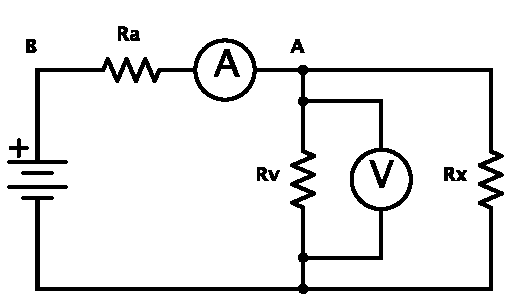
\includegraphics[width=\textwidth]{R_monte.pdf}
        \caption{Schema del circuito con amperometro a monte.}
        \label{fig:monte}
    \end{subfigure}%
    ~~ %add desired spacing between images, e. g. ~, \quad, \qquad etc.
      %(or a blank line to force the subfigure onto a new line)
    \begin{subfigure}[h!]{0.3\textwidth}
        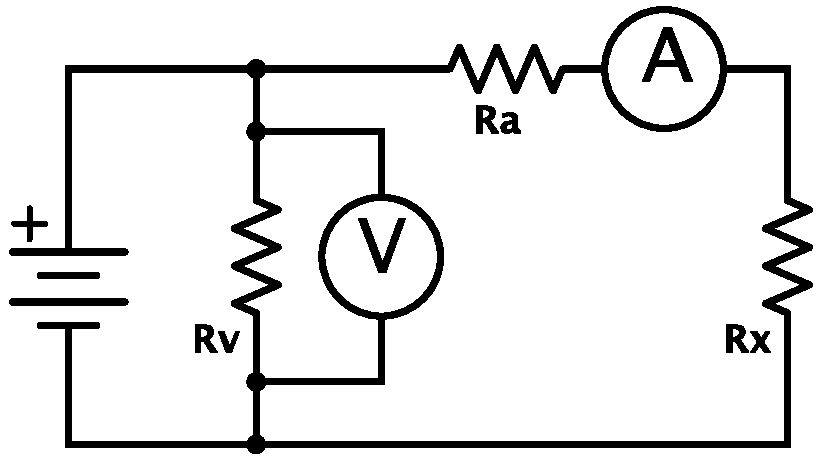
\includegraphics[width=\textwidth]{R_valle.pdf}
        \caption{Schema del circuito con amperometro a valle.}
        \label{fig:valle}
    \end{subfigure}%
    \caption{Schemi circuitali utilizzati.}
    \label{fig:circuiti}
\end{wrapfigure}


\section{Strumenti}

$\bullet \quad$7 resistenze:\\
\phantom{x}$\quad$1, 10, 100, 1k, 10k, 100k, 1M$\Omega$\\
$\bullet \quad$Cablaggio\\
$\bullet \quad$2 tester ICE\\
$\bullet \quad$Generatore di corrente DC\\
$\bullet \quad$Multimetro digitale\\
$\bullet \quad$Breadboard (basetta sperimentale)\\